\newprob{1718634071}
{
    含鈾岩石在形成之初並不含任何氦原子。含鈾岩 石形成後,當中的鈾238(U-238)會進行以下的 衰變,最後形成穩定的鉛206 (Pb-206)。
    % \par{\par\centering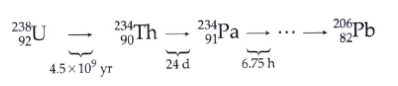
\includegraphics[width=.6\textwidth]{./img/ch2_decay_lq_2024-06-17-22-23-39.png}\par}
    \begin{align*}
        \ce{^{238}_{92}U ->[][ \qty{4.5e9}{yr}] ^{234}_{90}Th ->[][ \qty{24}{d}] ^{234}_{91}Pa ->[][ \qty{6.75}{h}] $\dots$ -> ^{206}_{82}Pb}
    \end{align*}
    在以上衰變中,首個衰變(從鈾238 至釷234)比 其餘隨後的衰變需時都要更久。因此,以上衰變 系可簡化成一個從鈾238 至鉛206的單一衰變, 其半衰期約 \num{4.5e9}年。
    % \par{\par\centering
\includegraphics[width=.6\textwidth]{./img/ch2_decay_lq_2024-06-17-22-24-27.png}\par}
    \begin{align*}
        \ce{^{238}_{92}U ->[][ \qty{4.5e9}{yr}]  ^{206}_{82}Pb}
    \end{align*}
    在此衰變中,一顆鈾原子衰變至鉛原子,一共會 釋放8顆$\alpha$粒子。 \\現為某個含鈾岩石的樣本進行檢驗,發現當中的 鈾原子和氦原子之比為$15:8$,試估計該岩石樣 本的年齡。\zzh{3}
}{
    \src{Active Physics p79 q7}
    \par{\par\centering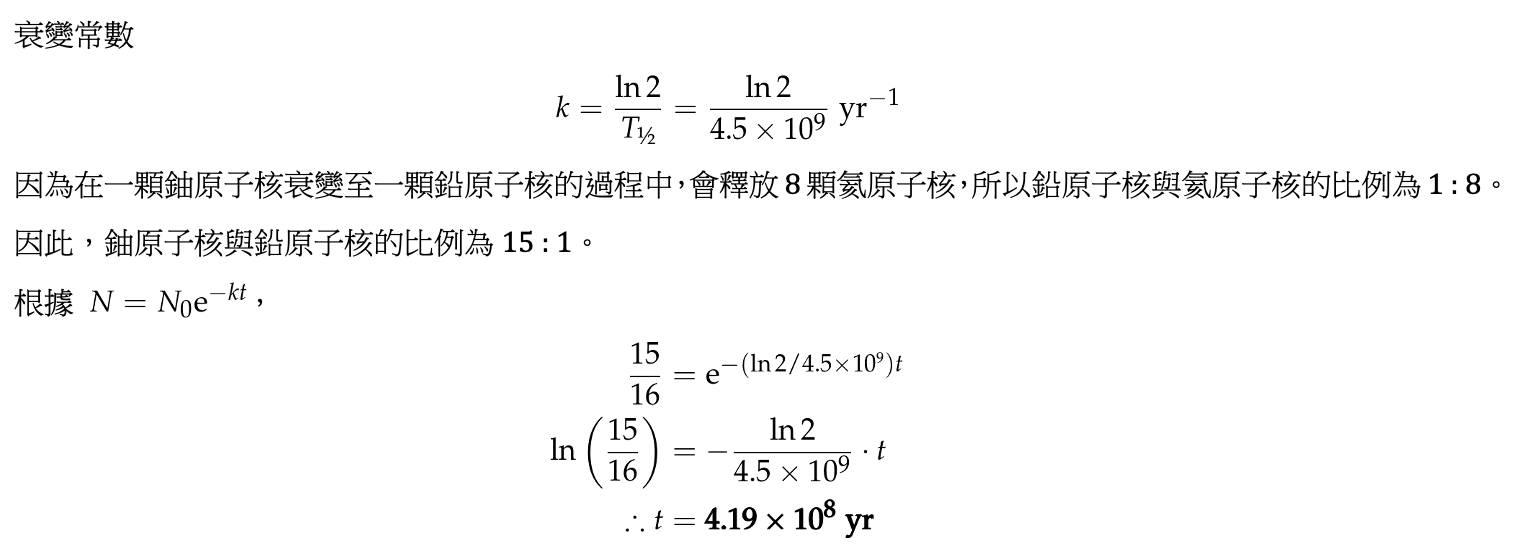
\includegraphics[width=\textwidth]{./img/ch2_decay_lq_2024-06-17-23-10-03.png}\par}
}

\newprob{1718634349}
{
    明樂在學校實驗室中進行放射實驗。實驗所用的 放射源存放在一個容器內。
    \begin{parts}
        \part 該容器應以甚麼物料製造(木、鋁還是鉛)? 為甚麼? \zzh{2}
        \part 實驗所用的放射源會放出$\alpha$ 和$\gamma$輻射。在 下列情況中,哪種輻射會對明樂造成較大傷 害? \zzh{2}
        \begin{subparts}
            \subpart 明樂意外地攝入放射源。
            \subpart 明樂的皮膚曾與放射源接觸。
        \end{subparts}
        試扼要解釋你的答案。
        \part 舉出\textbf{兩項}處理放射源應採取的安全措施。 \zzh{2}
    \end{parts}
}{
    \src{Active Physics p85 q4}
    \par{\par\centering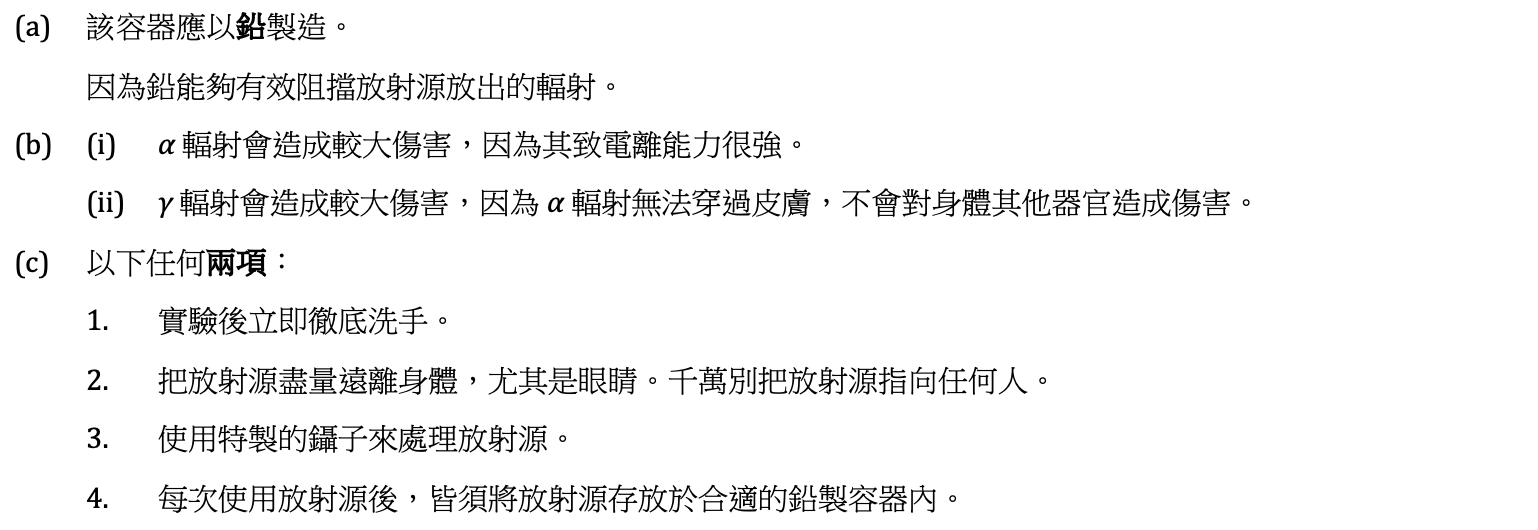
\includegraphics[width=\textwidth]{./img/ch2_decay_lq_2024-06-17-23-08-12.png}\par}
}

\newprob{1718634528}
{
    放射性同位素鈷60(Co-60)的半衰期為5.27年。 某樣本起初含有  \qty{0.2}{\mu g} 的純Co-60。
    已知:阿佛加德羅常數 =  \qty{6.02e23}{mol^{-1}} \\
    1年 =  \qty{3.15e7}{s} \\
    1 摩爾鈷 60 的質量 = 60 g
    \begin{parts}
        \part 起初,樣本中未衰變原子核的數目為多少?\zzh{2}
        \part 衰變常數的物理意義是甚麼?求Co-60的衰 變常數。 \zzh{3}
        \part 起初,樣本的放射強度為多少?\zzh{2}
        \part 估計樣本中未衰變原子核的數目減少至原來 的$10\%$ 需時多久。 \zzh{2}
    \end{parts}
}{
    \src{Active Physics p89 q11}
    \par{\par\centering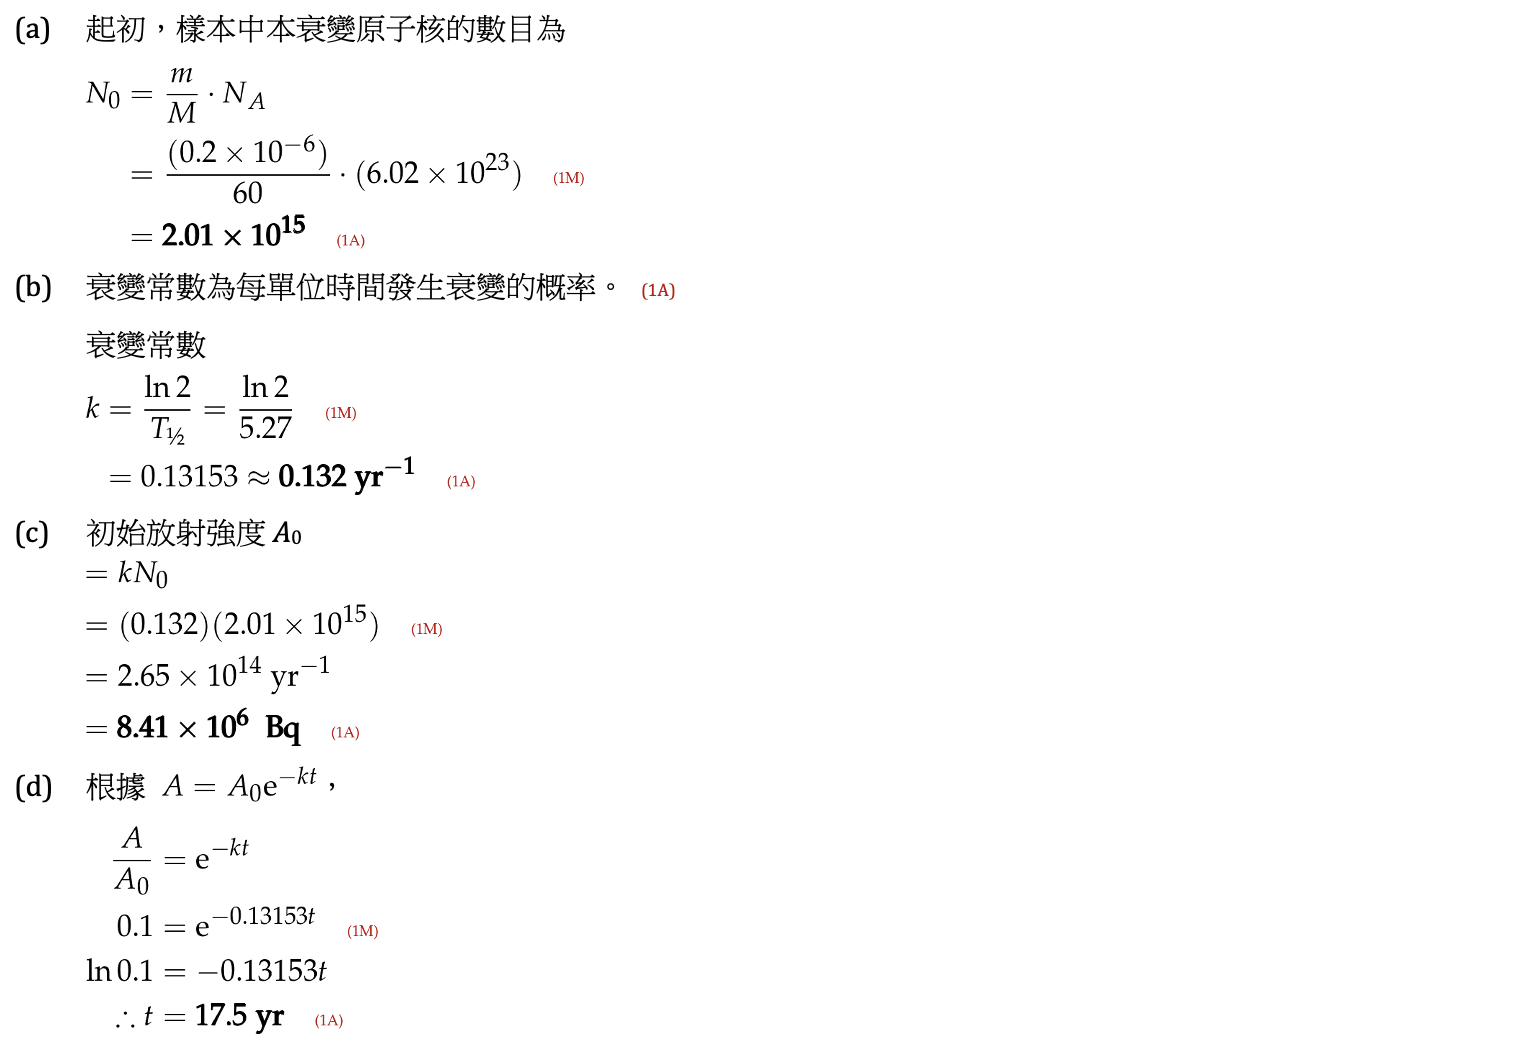
\includegraphics[width=\textwidth]{./img/ch2_decay_lq_2024-06-17-23-07-47.png}\par}
}

\newprob{1718636038}
{
    一個樣本含有放射性核素$X$和$Y$,兩者的衰變曲 線如下圖所示。
    \par{\par\centering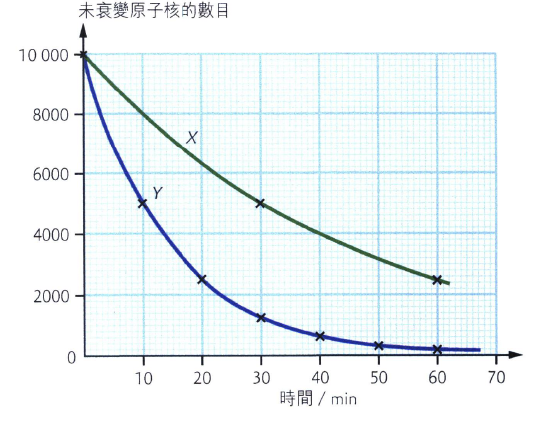
\includegraphics[width=.6\textwidth]{./img/ch2_decay_lq_2024-06-17-22-54-20.png}\par}
    \begin{parts}
        \part 半衰期的意義是甚麽?\zzh{1}
        \part 試判斷放射性核素X和Y的半衰期。\zzh{2}
        \part 求$X$和$Y$的衰變常數。\zzh{3}
        \part 求樣本在時間為25 min 時的放射強度。\zzh{4}
    \end{parts}
}{
    \src{Active Physics p89 q13}
    \par{\par\centering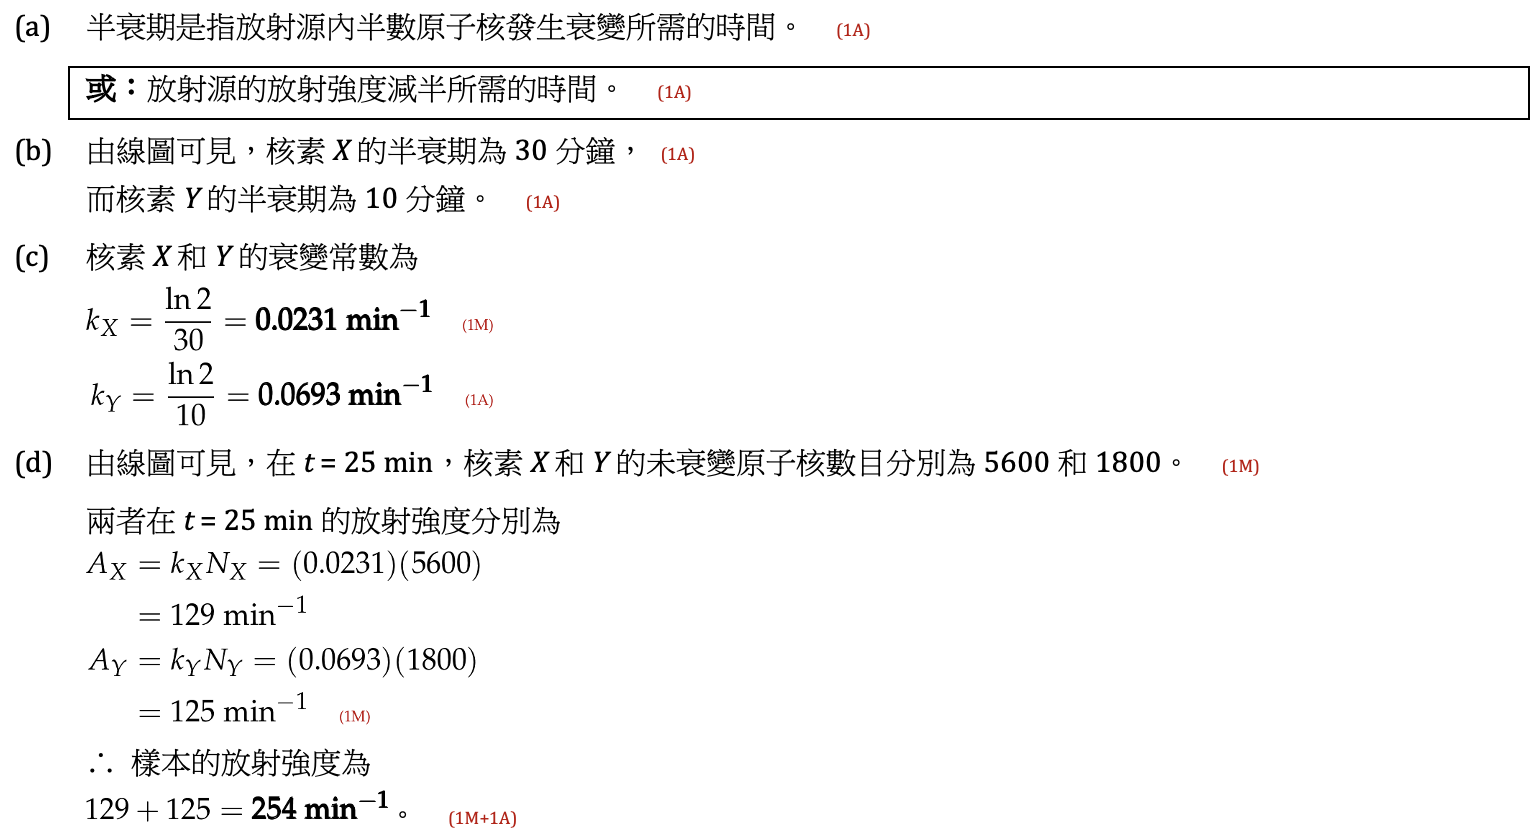
\includegraphics[width=\textwidth]{./img/ch2_decay_lq_2024-06-17-23-07-32.png}\par}
}

\newprob{1718636120}
{
    下圖顯示一個監測聚苯乙烯片厚度的機器。接受 檢測的聚苯乙烯片會通過放射源和探測器之間。 已知放射源放出$\beta$輻射。
    \par{\par\centering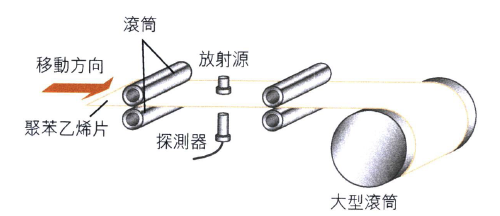
\includegraphics[width=.5\textwidth]{./img/ch2_decay_lq_2024-06-17-22-55-43.png}\par}
    \begin{parts}
        \part
        為甚麼$\alpha$ 和$\gamma$放射源對這台機器來說並不適 用? \zzh{2}
        \part 放射源的半衰期應為長或短?試扼要解釋。\zzh{2}
        \part 下表顯示計數器的讀數隨時間的變化。
        \par{\par\centering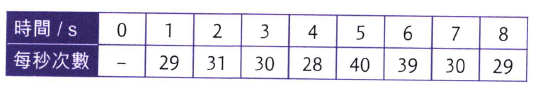
\includegraphics[width=.6\textwidth]{./img/ch2_decay_lq_2024-06-17-22-57-56.png}\par}
        根據以上資料,簡單描述聚苯乙烯片的厚度 變化。 \zzh{2}
    \end{parts}
}{
    \src{Active Physics p89 q15}
    % \par{\par\centering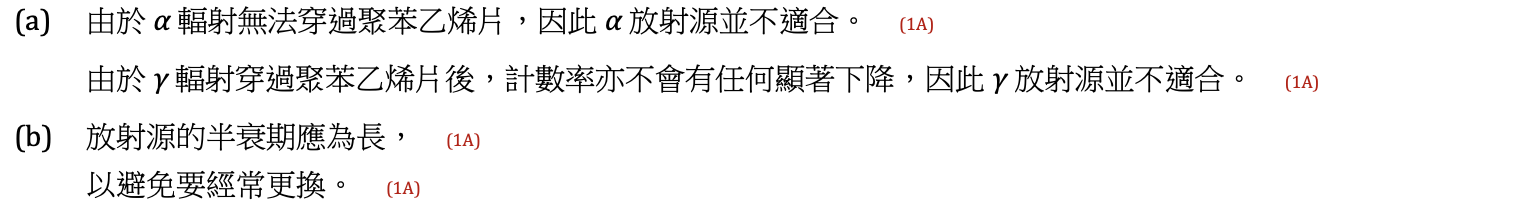
\includegraphics[width=\textwidth]{./img/ch2_decay_lq_2024-06-17-23-07-19.png}\par}
    \par{\par\centering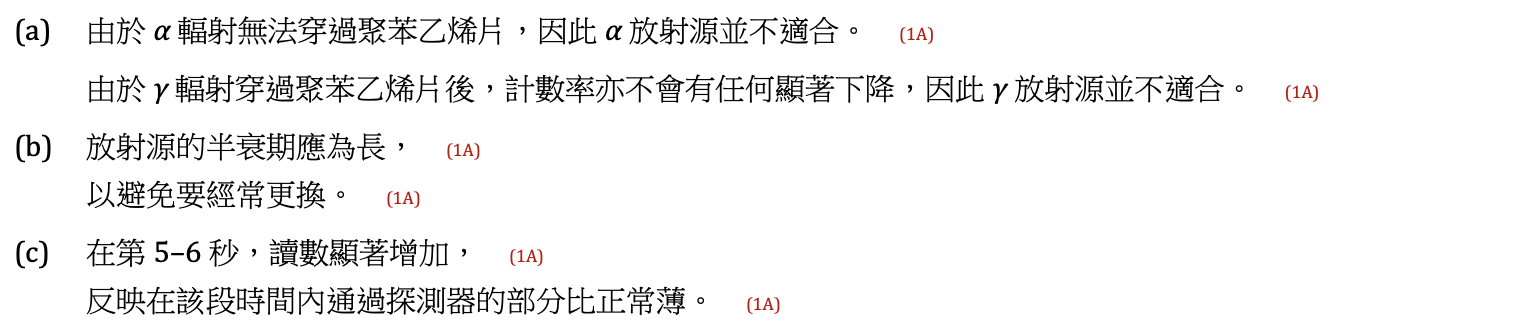
\includegraphics[width=\textwidth]{./img/ch2_decay_lq_2024-06-17-23-21-21.png}\par}
}

\newprob{1718636317}
{
    一個放射性樣本在不同時間$t$的放射強度$A$可用 方程 $A=A_0\textrm{e}^{-kt}$來描述。以下為$\ln A$對$t$的關係線圖。
    \par{\par\centering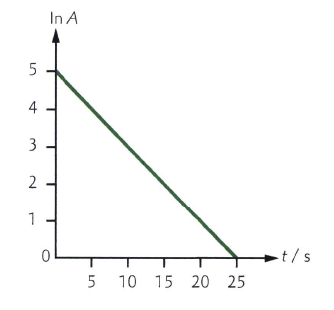
\includegraphics[width=.4\textwidth]{./img/ch2_decay_lq_2024-06-17-23-01-22.png}\par}
    \begin{parts}
        \part 樣本的初始放射強度為多少?\zzh{2}
        \part 求半衰期。\zzh{3}
        \part 若放射源的半衰期較長,線圖會有甚麼不同?\zzh{1}
        \part 現考慮一個混有放射性物質$P$和$Q$的樣本。 在不同時間$t$,記下了該樣本的放射強度$A$。 線圖顯示 $\ln A$ 隨時間$t$的變化。
        \par{\par\centering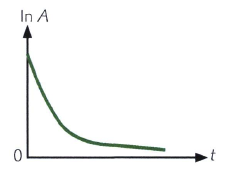
\includegraphics[width=.35\textwidth]{./img/ch2_decay_lq_2024-06-17-23-02-37.png}\par}
        已知$P$的半衰期遠比$Q$長,試扼要解釋曲線 兩端何以看起來像直線一般。 \zzh{2}
    \end{parts}
    \dlines{1}\clearpage
}{
    \src{Active Physics p91 q2}
    \par{\par\centering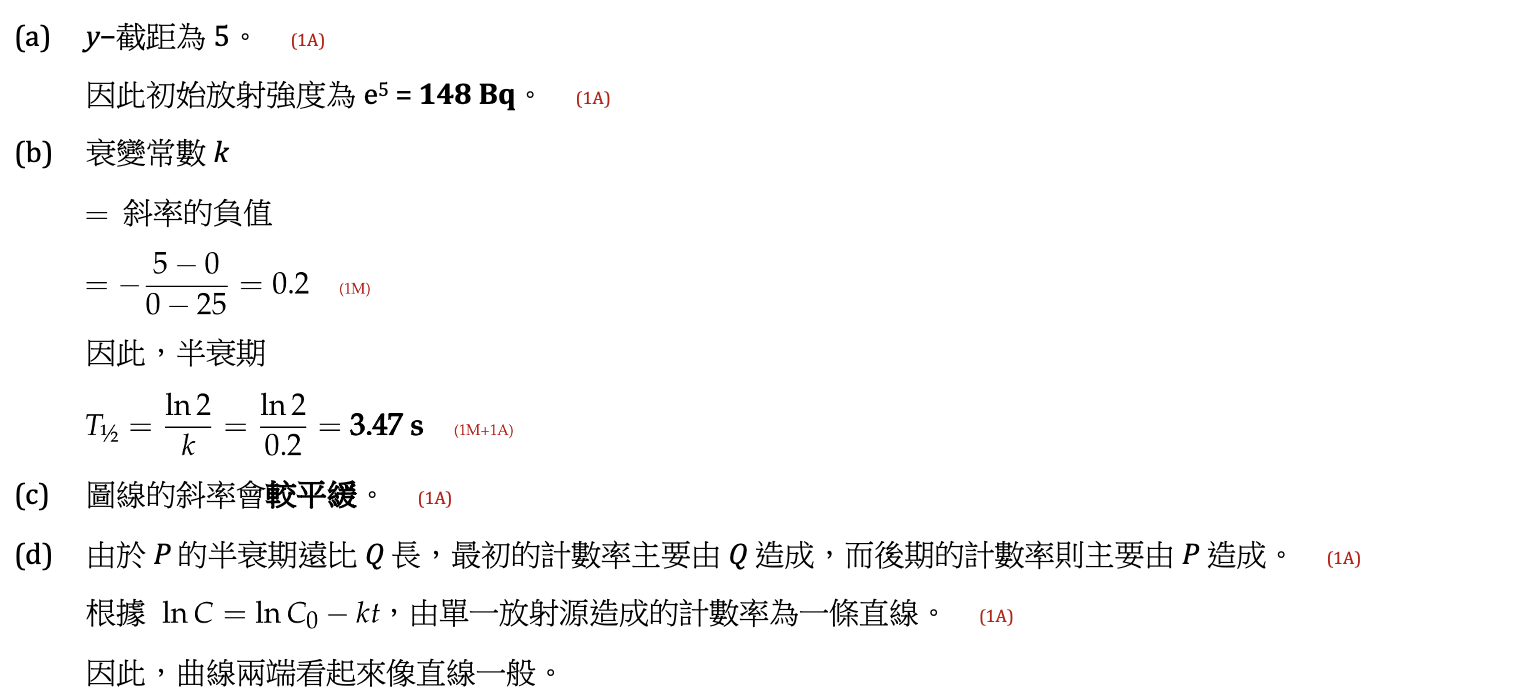
\includegraphics[width=\textwidth]{./img/ch2_decay_lq_2024-06-17-23-07-03.png}\par}
}